\documentclass[11pt]{article}
\usepackage[english]{babel}
\usepackage{enumitem}
\usepackage{fancyhdr}
\usepackage{amsfonts, amssymb}
\usepackage{graphicx}
\usepackage{caption}
%\usepackage[cm]{fullpage} %%formats everything to maximize space (can edit easily use wiki)
\usepackage{amsmath}   
\usepackage{avant}
\usepackage{graphicx}
\usepackage{amsthm}  %Theorem Stuff
 \usepackage{algpseudocode}
 \usepackage{tikz}
 \usepackage{url}
\usepackage[colorlinks, linkcolor=cyan, citecolor = cyan]{hyperref} %for table of contents
\usepackage[all]{hypcap}
\usepackage{sectsty} 
\usepackage[font = small, labelfont = bf, textfont= small]{caption}
\usepackage{subcaption, array}

%\allsectionsfont{\center \textsc}


 %%%%%%%%FANCYHEADER%%%%%%%%%%%

 

  %\setlength\parindent{0pt}
  
 \pagestyle{fancy}
 \headsep = 25pt %%%makes sure the header doesn't spill into the rest of the page.
 \fancyhf{} %delete the current section for header and footer
 \fancyhead[L]{}
 \fancyhead[L]{\today}
  \fancyhead[R]{Criminal Pursuit}
 \fancyfoot[C]{\thepage}




\newcommand{\chose}[2]{\left(\begin{array}{c}{#1} \\ {#2}\end{array}\right)}
\newcommand{\PI}{\textrm{PI}}
\newcommand{\BI}{\textrm{BI}}
\newcommand{\dist}{\textrm{dist}}
\renewcommand{\b}[1]{\mathbf{#1}}
\renewcommand{\c}[1]{\mathcal{#1}}
\renewcommand{\t }[1]{\mathrm{#1}}
\newcommand{\bb}[1]{\mathbb{#1}}
\newcommand{\bR}{\bb R}
\newcommand{\eps}{\varepsilon}
\renewcommand{\L}{\mathrm{L}}
\newcommand{\T}{\mathrm{T}}
\newcommand{\V}{\mathrm{V}}
\newcommand{\eqop}{=}
\renewcommand{\phi}{\varphi}
\renewcommand{\l}{\ell}
%\renewcommand{\rmdefault}{ppl} %Change the font

\tikzstyle{no1}=[circle, draw, fill = yellow!65!green, inner sep = .08 cm]
\tikzstyle{aux} =[ inner sep = .08 cm]
\tikzstyle{no2}=[circle, draw, fill = yellow!95!green, inner sep= .08 cm]
\tikzstyle{no3}=[circle, draw, fill = yellow!95!green, minimum size= .35 in]
\tikzstyle{no4}=[circle, draw, fill = yellow!65!green, minimum size= .35 in]
\title{Criminal Pursuit on a Preferential Attachment Tree}
\author{Charlie Z. Marshak, M. Puck Rombach, \\Andrea L. Bertozzi, and Maria R. D'Orsogna}
\theoremstyle{plain}
\newtheorem*{proposition}{Proposition} 
\theoremstyle{definition}
\newtheorem*{example}{Example}

\def\changemargin#1#2{\list{}{\rightmargin#2\leftmargin#1}\item[]}
\let\endchangemargin=\endlist

%%%%%%%%%%%%%%%%%%%%%%%%%%%%%%%%%%%%%%%%%%%%%%%%%%%%%%%%%BEGIN TEXT HERE%%%%%%%%%%%%%%%%%%%%%%%%%%%%%%%%%%%%%%%%%%%%%%%%%%%%%%%%%%%%%%%%%%%%%%%%%%%%%%%%%%%%%%%%%%%%%%%

\begin{document}

\maketitle
\begin{center}{\textbf{\textsc{Abstract}}}\end{center}
\begin{changemargin}{15mm}{15mm} 
\begin{small}
We model the hierarchal evolution of an organized crime network under the competing influences of a kingpin and the police.  At each time step, the network's members incorporate new criminals into the network.  Additionally, an officer looks to arrest as many criminals, old and new, as she can, with the kingpin's arrest being the ultimate goal.  The growth process follows a preferential attachment model: criminals arrive at a constant rate and attach to existing criminals with probability roughly proportional to the inverse distance to the lowest level of the hierarchy.  Here, the lowest ranking criminals are those without any underlings.  Then, the officer follows a self-avoiding random walk and she can arrest criminals at any given moment in her pursuit.  Alternating between growth and pursuit fashions our dynamic graph model of an organized crime network.  For the growth process, we study the evolution of criminal rankings in the network and the degree distribution in the network as $t \to \infty$.  For the pursuit process, we numerically simulate the dynamic game and infer that a degree-threshold strategy for the police is optimal given that the officer's knowledge is confined to local network data.
\end{small}

\end{changemargin}
\section*{Introduction}

Network science has become a central tool in the modeling of criminal behavior \cite{mcIllwain, browning, tita}.  Haeurt and his collaborators paired networks and evolutionary game theory to model human cooperation within a Darwinian framework \cite{Hauert1, Hauert2, Hauert3}.  The joint work of the last author with Short and Brantingham employed similar ideas to model the interplay of criminals and informants in society \cite{maria2010, maria2012}, and then with the addition of a social network apparati by Short, et al. \cite{mccallaEGT}.   Using these models as a springboard, we model the dynamics of a hierarchal crime network that undergoes expansion via recruitment and then shrinkage due to arrest.  The tree structure is an appropriate choice for networks that are large and entrepreneurial in nature \cite{crime1, crime2}.  Our model has two key components: network growth and police pursuit.\\  
\\
The first component of the process, the growth, introduces a preferential attachment mechanism that follows in spirit of the mathematical work of Szyma\'{n}ski \cite{sz}, Yule \cite{Yule}, Barab\'{a}si-Albert \cite{BA1}, and Mahmoud \cite{Mahmoud1, Mahmoud2}.  This growth process models criminal recruitment.  Criminals are added to the network at a constant rate and each form a unique connection to the existing network.  In criminology, recruitment into a criminal network is a complicated process that involves both the recruiter and the network to acquire trust and to engage in frequent communication \cite{recruitment1, recruitment2}.  In this mathematical simulation of recruitment, we model the recruitment probabilistically and attempt to capture some of the human elements.  We assume the incoming criminals will most likely form a link to those with closest ties to street activity because criminological studies suggest prospective members of a criminal network are those already engaged in illicit street activities themselves \cite{recruitment1}.  Also, those criminals without underlings will have more more time to communicate to prospective criminals and are likely the most visible to people outside of the network.  Again, proximity to street crime in our network model is understood in terms of the minimum distance a criminal is from any of the other criminals without underlings.\\
\\
We remark, that in our model, while street criminals are the most likely to recruit, even the kingpin can form a link to a prospective throughout the life of the network, though the probability this occurs will become small as the network grows large.  Due to the possibility of investigation and arrest, which will be formally introduced as a graph game later, criminals benefit from maintaining a buffer between themselves and street criminals in the network.   The more recruiting any criminal does, the more vulnerable and visible she is to police capture.  Thus, long-time members of the network should have less incentive to recruit, which is reflected in their low probability of adding a link.\\
\\
The second component of the process, the pursuit, adapts the classic ``birth-death" apparatus from population dynamics \cite{kendall, gardiner} into this criminal network model.  We detail the movement of a single officer whose ultimate goal is to capture the kingpin.  The officer proceeds by a self-avoiding random walk beginning with one of criminals without underlings.  If she arrives at the kingpin, then the pursuit is successful and the process is terminated.  If the officer can no longer move, then the pursuit is unsuccessful and the officer must attempt to capture the kingpin the next round.  At any point in the investigation, the officer can arrest the criminal she is currently investigating and all of the criminals below.  By removing criminals from the network, the officer makes the kingpin more vulnerable to future capture.\\
\\
We view the process as a game on a graph with the two players represented by a kingpin and an officer.  The kingpin wins if the officer does not capture the kingpin in finite time and the officer wins otherwise.  We study strategies for arrest that the officer can pursue.


\section*{Part I: Preferential Attachment}


Let $\t T^{(0)}$ be the initial criminal network with unique kingpin.  Set $\t T^{(t)}$ to be a recursively defined network at time $t$ with $\V^{(t)}$ the set of criminals.  The set of criminals $\L^{(t)}$ contained in $\V^{(t)}$ denotes those criminals without any underlings.  We assume $\L^{(t)}$ are the criminals closest to street activity.  To obtain $\t T^{(t)}$ from $\t T^{(t-1)}$, we add $k$ new criminals to $\t T^{(t-1)}$; we call $k$ the rate of new criminal arrival . Let $\dist_t(j)$ denote the minimum distance from criminal $j$ to $\L^{(t)}$.  Each new criminal forms a link to an existing criminal $j$ on $\t T^{(t-1)}$ with probability proportional to weight $w_{t-1}(j)$.   In particular, if a new criminal $i$ is added to the tree $\t T^{(t)}$, then the probability that an edge $e_{ij}$ from $i$ to $j$ is formed is given by:
$$
\bb{P}_t(e_{ij}) = \frac{w_{t-1}(j)}{\sum_{j'} w_{t-1}(j')}
$$
The weight $w_t(j)$ of criminal $j$ at time $t$ is defined as:
\begin{align*}
w_t(j)  &:= \frac{1}{\dist_t(j)+A}
\end{align*}
with $A\in \b R$.  We set $A = 1$ for this model.  Observe that $0 \leq w_t(j) \leq 1$ for all $j \in \V^{(t)}$ and the maximum of $w_t$ is attained for $j \in \L^{(t)}$.  See Figure [\ref{grow1}] for an illustration of the probability assigned to each criminal for a given experiment.  We remark that as $A \to \infty$, $w_t(j)$ is a uniform weight on each of the nodes and the process becomes the recursive trees found in \cite{Mahmoud1, Mahmoud2, sz}.  As $A \to 0$, criminals with higher and higher probability link to criminals without underlings and the model will become increasingly deterministic.  Our decision to use $A  = 1$ stems from the fact that we wish to have a middle ground between these two extremes: more weight should be given to criminals without underlings, while still permitting long-standing criminals to have a chance of forming a new criminal link.

\begin{figure}\centering
\title{\bf{Preferential Attachment, $t = 0, 1,2$}}\\
\vspace{.5 cm}
 \begin{subfigure}[b]{.12 \textwidth}\centering
 \begin{small}
 \begin{tikzpicture}[level distance=2.5cm, scale = .75]
  \tikzstyle{level 1}=[sibling distance=3cm];
  \node[no1, label= south:{$\bb{P}_0\eqop 1$}] (root) {};
\end{tikzpicture}
\end{small}
\vspace{1.5 cm}
  \caption{$t = 0$}
  \end{subfigure}
    \hspace{.25 cm}
 %%%%%%%%%%%%%%%%%%%%%%%%%%%%%%%%%%%%%%%%%%%%%%%%%%%%%%%%%%%%%%
   \begin{subfigure}[b]{.3\textwidth}\centering
   \begin{small}
\begin{tikzpicture}[level distance=1.5cm, scale = .75]
  \tikzstyle{level 1}=[sibling distance=1cm];
  \node[no1, label = {[label distance=-0.25 cm]30:$\begin{matrix} \bb{P}_2\approx\\  0.{14}\end{matrix}$}] (root) {}
   [no1, ]
     child {node[no2, label={[label distance=-0.2cm]170:$ \begin{matrix}\bb{P}_1 \approx\\ 0.29\end{matrix}$ }] {}
      }
child  {node [no2, label=   {[label distance=-.25cm]270 :$ \begin{matrix}\bb{P}_1 \approx\\ 0.29\end{matrix}$}]{}
     }
  child  {node [no2, label={[label distance=-0.25cm]0:$ \begin{matrix}\bb{P}_1 \approx\\ 0.29\end{matrix}$}]{}
           };
\end{tikzpicture}
\end{small}
\caption{$t = 1$}
  \end{subfigure}
  \hspace{.25 cm}
  %%%%%%%%%%%%%%%%%%%%%%%%%%%%%%%%%%%%%%%%%%%%%%%%%%%%%%%%%%%%%%
  \begin{subfigure}[b]{.3\textwidth}
  \begin{small}
  \centering
\begin{tikzpicture}[level distance=1.5cm, scale = .75]
  \tikzstyle{level 1}=[sibling distance=2cm];
  \tikzstyle{level 2}=[sibling distance=1.5cm];
  \node[no1, label = {[label distance=-0.25 cm]30:$\begin{matrix} \bb{P}_2\approx\\  0.{18}\end{matrix}$}] (root) {}
   [no1, ]
     child {node[no1, label= west:$\begin{matrix}\bb{P}_2 \approx\\  0. {09}\end{matrix}$ ] {}
       child  {  node[no2, label = {[label distance=0 cm]190 :$\begin{matrix} \bb{P}_2\approx\\  0.{18}\end{matrix}$}]{}
		}
      }
child  {node [no1, label={[label distance=-.35cm]180:$\begin{matrix}\bb{P}_2 \approx\\  0. {09}\end{matrix}$}]{}
       child {node[no2, label=   {[label distance=-0.25cm]-90 :$\begin{matrix}  \bb{P}_2 \approx\\ 0.{18}\end{matrix}$}] {}}
       child {node [no2, label=  {[label distance=-.3cm]0: $\begin{matrix} \bb{P}_2 \approx\\ 0.{18}\end{matrix}$}]{}}}
  child  {node [no1, label= {[label distance=-.1cm]90:$\begin{matrix}\bb{P}_2 \approx\\ 0.{18}\end{matrix}$}]{}};
\end{tikzpicture}
\end{small}
\caption{$t= 2$}
%%%%%%%%%%%%%%%%%%%%%%%%%%%%%%%%%%%%%%%%%%%%%%%%%%%%%%%%%%%%%%
  \end{subfigure}

\caption{The above figure shows $\bb P_{t+1}$, the probability a new link is formed to one of the $k$ new criminals entering the network .  Here, the rate of criminal arrival $k$ is $3$ and $\mathrm{T}^{(0)}$ is the kingpin alone.  To calculate $\bb P_{t+1}$, we must find $d_t$, the distance a criminal is from $\L^{(t)}$ and then $w_t$, the weight of the criminal $i$ at $t$ given by $\frac 1{d_t+1}$.  Lighter green leaves denotes criminals new to the network on the given time step.}
\label{grow1}
\end{figure}

\begin{table}\centering
\begin{tabular}{|m{5.75cm}|m{5.75cm}|}
\hline
This Model's Terminology&Network Theory Terminology\\
\hline
\hline
The kingpin& The root\\
\hline
$\T^{(t)}$: Criminal Network& A rooted tree at time $t$\\
\hline
$\V^{(t)}$: Criminals & Verticies or nodes at time $t$\\
\hline
$\L^{(t)}$: Criminals without underlings or street criminals& The set of leaves in the network at time $t$\\
\hline
\end{tabular}
\caption{Above, we provide a dictionary of the criminal network terminology used in this paper and that of standard network theory.}
\end{table}
 %%%%%%%%%%%%%%%%%%%%%%%%%%%%%%%%%%%%%%%%%%%%%%%%%%%%%%%%%%%%%%
\begin{table}\centering
  \begin{tabular}{|m{2cm}|p{9.75cm}|}
\hline
Parameter&Description\\
\hline
\hline
$t$& Time\\
\hline
$k$ & New criminals added to the network at each timestep\\
\hline
$\T^{(0)}$& Initial network configuration\\
\hline
$A$& Parameter in $w_t(j)$.  We set $A = 1$.\\
\hline
$N$& Number of criminals before growth experiment stopped\\
\hline
\end{tabular}
  \caption{We record the parameters of the growth model above.}
\end{table}

  
  
\subsection*{Degree Distribution}

\begin{figure}
\centering
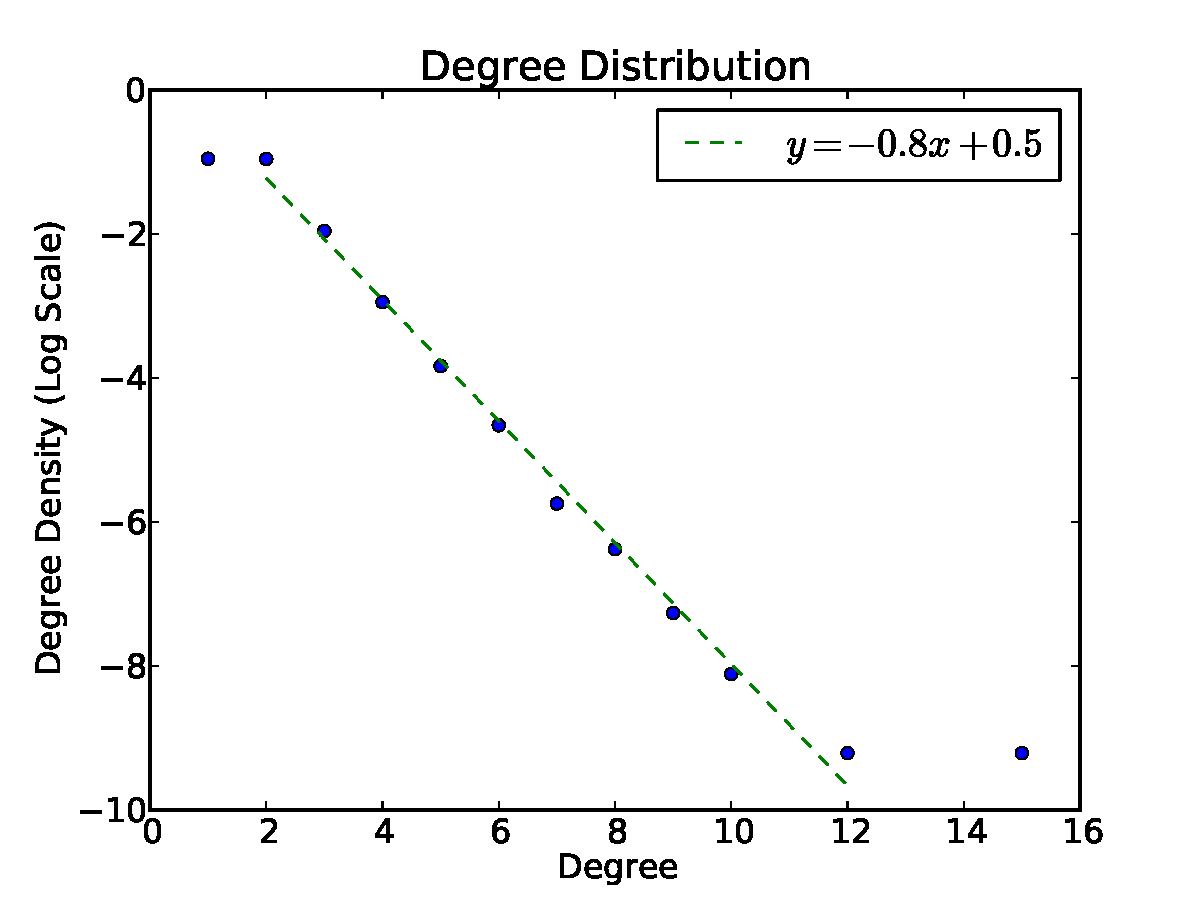
\includegraphics[width=.75\linewidth]{DegDist.pdf}
\caption{The Criminal Network was grown to 10000 (N).  500 experiments were performed, averaged, and then collected into a histogram. Observe that the number criminal with 1 and 2 degree are roughly at the same proportion.  The criminals of degree 1 are precisely the criminals without underlings, or street criminals.  The criminals of degree 2 are with high probability those criminals a distance 1 from the aforementioned street criminals.  These two populations represent the pipeline into the network and it makes sense that these two populations occupy the same proportion for all time.  The tail of the distribution, those criminals with high degree, picks up noise on account of its rarity.  The fit becomes more and more pronounced as $N \to \infty$ and the number of experiments increases.}
\label{DD}
\end{figure}

The Barab\'{a}si-Albert model is a preferential attachment model, where nodes are added with greatest probability to network nodes of high degree \cite{bollscalefree, BA1} and is summarized as a network where ``the rich get richer".  A salient mathematical feature of this preferential attachment model is its heavy-tailed degree distribution, which obeys a power-law \cite{bollscalefree}.  From the data seen in Figure [\ref{DD}], we conjecture the degrees in this model are also heavy-tailed, and further, obey an exponential law with a shift.  While the empirical exponential law is difficult to numerically capture via numerical experiments \cite{powerlawempi}, we argue why there should be such a law heuristically.  When criminal adds a new link, then effectively a new network process begins.  This self-similarity permits a high probability that criminal degrees remain at a fixed proportion throughout the life of the network.

\subsection*{Criminal Density}

We found the criminal density depends on their distance to the kingpin.  Figure [\ref{nd}] suggested a shifted gamma ($\gamma$-) density numerically approximates this relationship.  As $N$ grows, the expected distance from the kingpin increases, which align's with the kingpin's desire to ensure a buffer between the possible police investigations of street criminals when the graph game begins.  The probability density of a $\gamma$-distributed random variable is given by:
$$
\rho_{\alpha, \beta, s}(h) = \frac{\beta^\alpha}{\Gamma(\alpha)}(h - s)^{\alpha-1}e^{ -\beta (h-s)}\quad h \geq 0.
$$
and if $X=$ distance to kingpin of a randomly selected criminal, then
$$
\bb P(X \leq h_0) \approx \int_{0}^{h_0}\rho_{\alpha, \beta, s}(h) \; dh
$$
Above, $h$ and $h_0$ denote distances to the kingpin.

\begin{figure}
\centering
\includegraphics[width=0.75\linewidth]{nodedensity.pdf}
\caption{The number of criminals $N$ in the network simulations were $2000, \; 4000$; and $6000$.  We fixed the arrival rate to be $k = 4$.  Our data is generated from 20 experiments.  $\t T^{(0)}$ was a complete tertiary tree of height 3.  We fit the data with a shifted $\gamma$-density.}
\label{nd}
\end{figure}
\subsection*{The Growth of Street Criminals}
Street criminals are those criminals without any underlings.  They have the highest probability of recruiting new criminals.  We assume street criminals are those primarily responsible for personally carrying out the illegal activity that permit the network to profit and whose presence make the streets more dangerous to network outsiders.  From a modeling perspective, we expect as the network grows, so too should the aggregate number of street criminals.  Set $\l(t) = |\L^{(t)}| =$ the number of street criminals at time $t$.  Then, Figure \ref{leaf} suggests that $\l(t)$ is linear in $t$ and that $\frac{d \l}{d t} = c_k$ is a constant that depends on $k$ alone.  The positivity agrees with our expectation that street criminals grow as the network does.  It also agrees with the fact that criminals of degree 1 remain at fixed proportion through the life of the network as the rate of criminal arrival $k$ is constant (see Figure \ref{DD}).

 \begin{figure}
 \centering
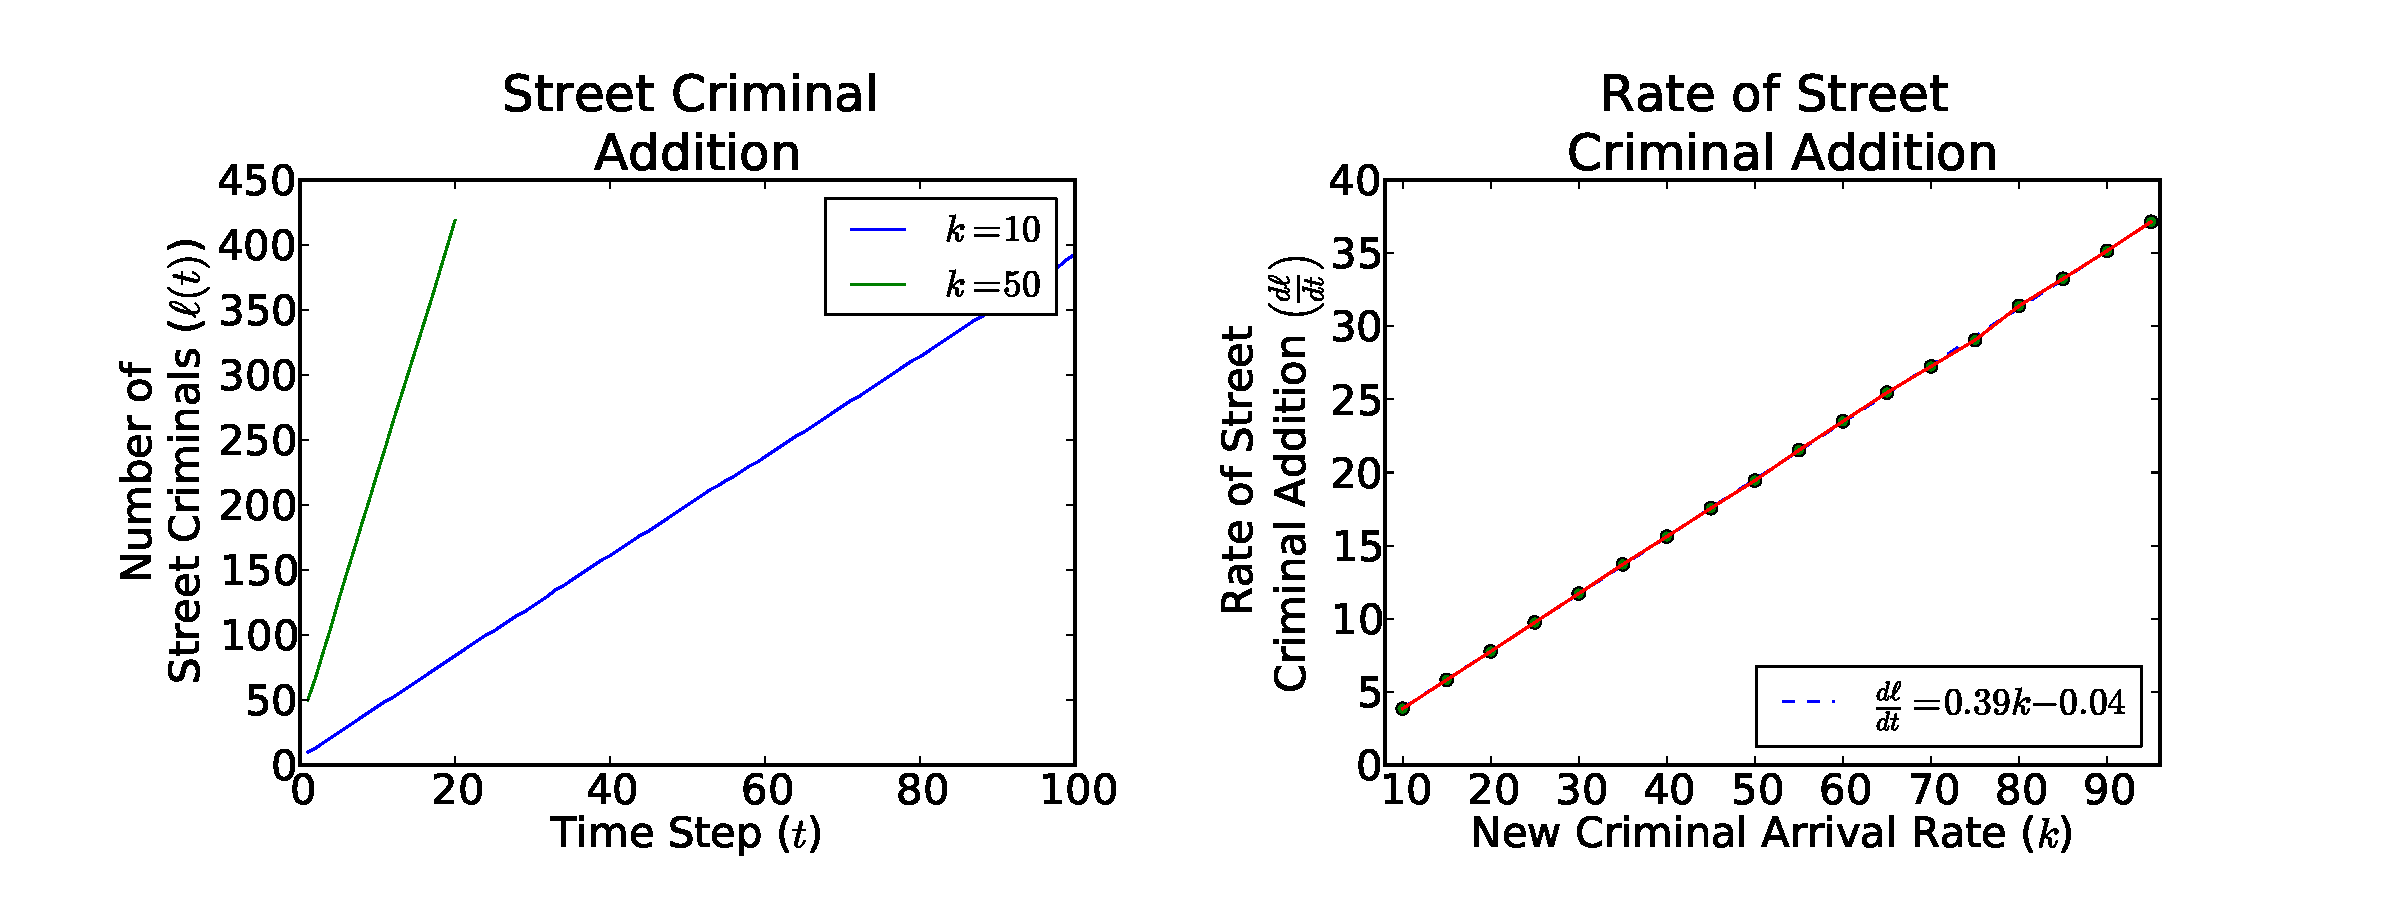
\includegraphics[width=\linewidth]{leafstats.pdf}
\caption{The number of criminals was fixed to be $N = 1000$, while $k$ was varied.  The function $\l(t)$ appears linear; moreover, the slope of this relation appears to linearly depend on $k$, i.e. $d \l/d t = c_k\approx .39k$. (right).}
\label{leaf}
\end{figure}


\subsection*{Network Proximity to Street Criminals}

The model has the feature that each criminal in the network is never too far removed from street activity.  In other words, all criminals have at least one path that connects them to another criminal in $\L^{(t)}$.  This effectively gives even the longest standing criminals in the network some access to the street as well as makes all criminals vulnerable to police intervention.  We can view
$$D_t:= \displaystyle{\max_{j \in \V^{(t)}} d_t(j)},$$
 as a random variable on $\T^{(t)}$ for any $t$.\\
\\
We predict $D_t$ to be bounded in the limit; that is, there exists an $M>0$ such that
$$\lim_{t \to \infty}\bb P( D_t\leq M) =1$$
assuming the limit exists.  As indicated by Figure \ref{harmseries},
$$ 
P\left(D_t > n\right) \leq \frac{1}{1+ \hdots + \frac{1}{n}}
$$
for a particular $\T^{(t)}$. 
\begin{figure}
\centering
\begin{tikzpicture}[scale = .65]
\node (a') at (-.0,3) [circle, fill = black!20, inner sep = .27cm] {};
\node (d') at (-1.5, .00) [circle, fill = black!20, inner sep = .27cm] {};
%\draw (b') to (c');
\draw [line width = .765 cm, color = black!20](0, 3) to (-1.5, 0);
\node (a) at (0, 3) [no1, thick] {};
\node (b) at (-.5, 2) [no1] {};
\node (c) at (-1, 1) [no1] {};
\node (d) at (-1.5, 0) [no1] {};
\node (e) at (-2, -1) [no2] {};
\node (aux1) at (.5, 2)[no2]{};
\node (aux2) at (0, 1)[no2]{};
\node(aux3) at (-.5, 0)[no2] {};
%%%%%%%%%%%%%%%%%%%%%%%
%%%%%%%%%%%%%%%%%%%%%%%
\draw (a) to (b);
\draw [dashed, thick](a) to (aux1);
\draw [dashed, thick](b) to (aux2);
\draw [dashed, thick](c) to (aux3);
\draw (b) to (c);
\draw (c) to (d);
\draw [dashed, thick] (d) to (e);
\end{tikzpicture}
\caption{Above the topmost node shows a criminal whose path realizes $D_t$, the maximum distance to $\L^{(t)}$; this path is highlighted in grey.  The light dashed edges denote possible connections a new criminal can make on this path.  Suppose the length of the path is $n$.  The probability the path will increase by 1 is $\frac{1}{ 1+ \frac 12 + \hdots + \frac 1n}$.}\label{harmseries}
\end{figure}
The boundedness is further inspected by numerical experiments found in Figure \ref{lw}.

\begin{figure}\centering
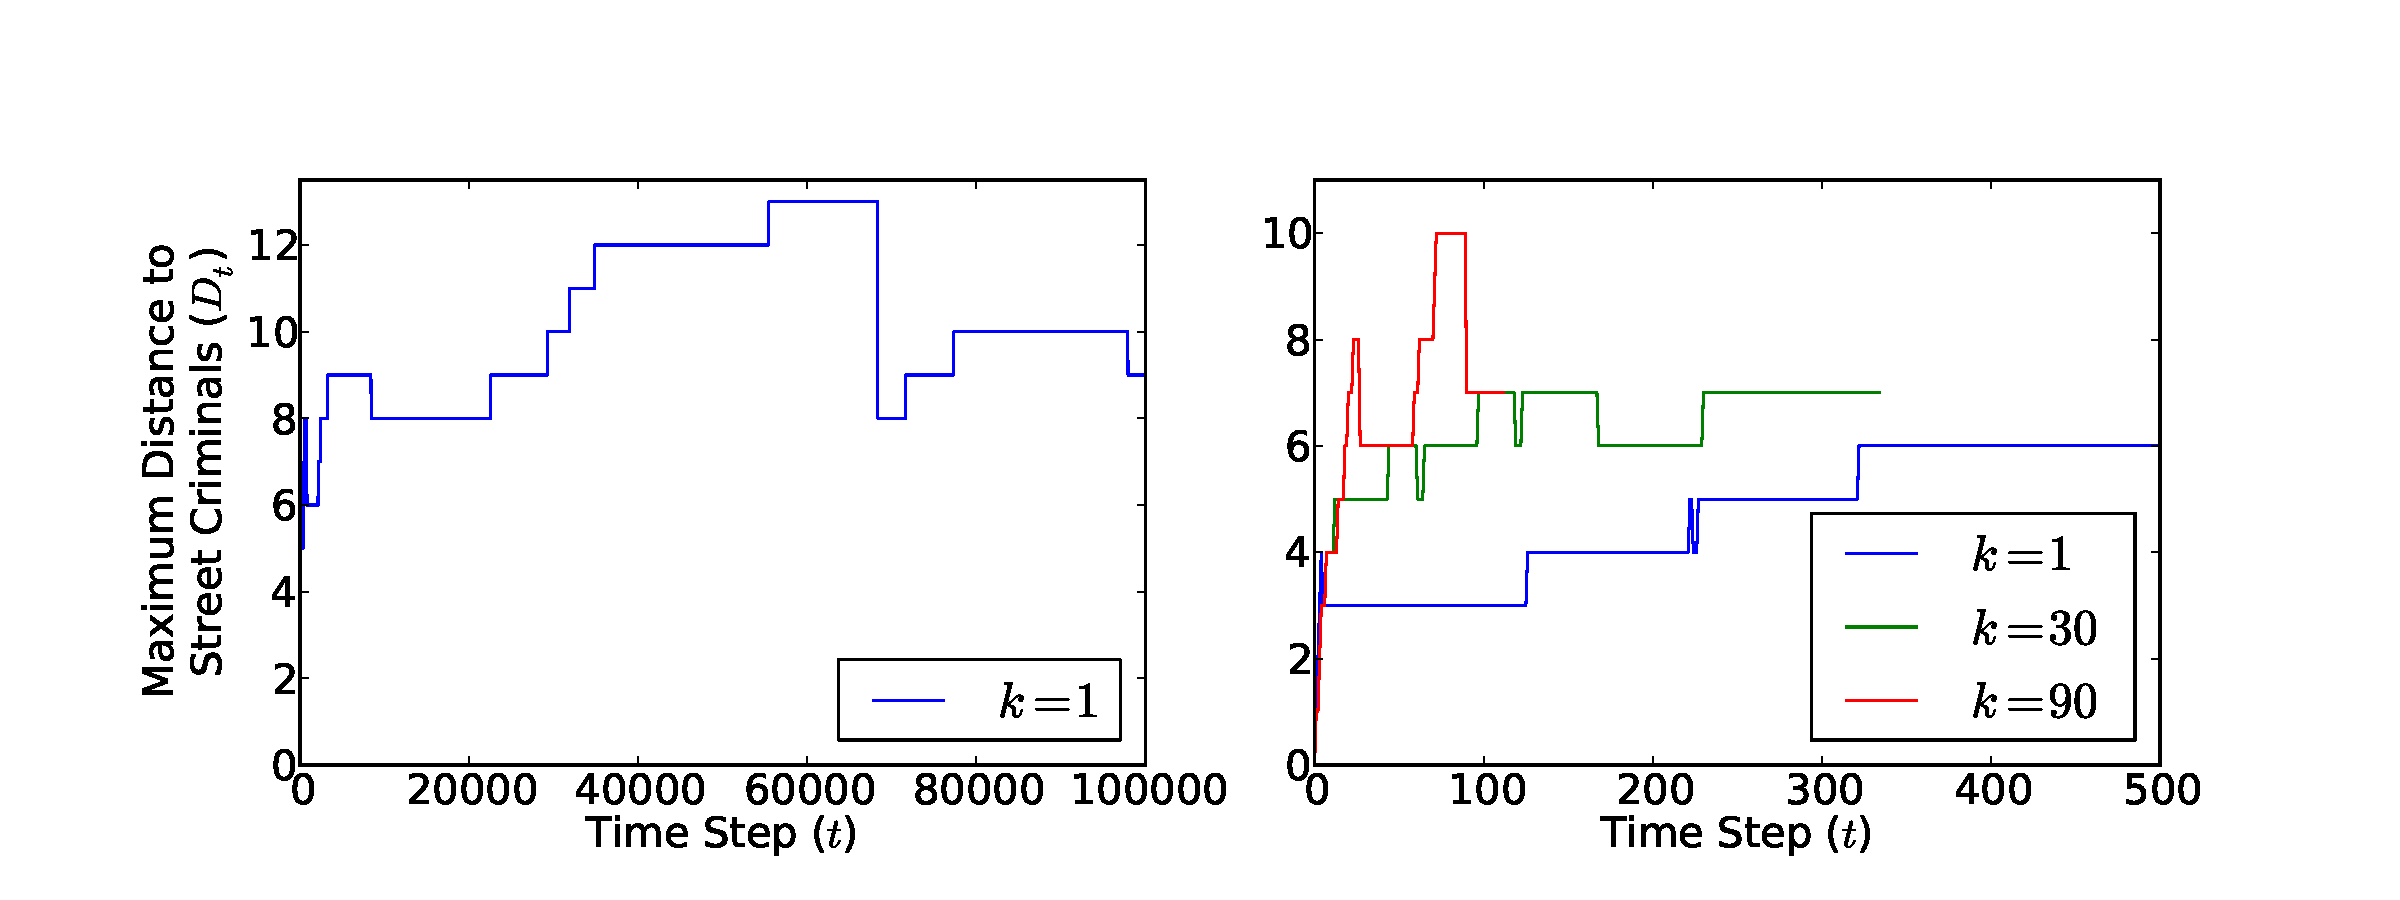
\includegraphics[width =  \textwidth]{LeafWatcher.pdf}
\caption{Above, we compute the maximum distance any criminal in the network is to a street criminal.  We inspect various criminal arrival rates $k$.  We see that for larger $k$, there is a sharper increase.  Even for a 100000 criminal network, $D_t$ appears to remain bounded.}
\label{lw}
\end{figure}
\section*{Part II: Adding Police Pursuit}

Once police pursuit is incorporated into the dynamics above, we view our process as a game with two players: the network led by a kingpin and the police led by a single officer.  A win for the officer is when she catches the kingpin in finite time.  A win for the network is precisely the opposite.

\subsection*{The Model with Police}
Let $\t T^{(0)}$ be the criminal network at $t =0$, one sufficiently large so that a win for the police is not inevitable.  We define a recursive process to obtain $\t T^{(t)}$ from $\t T^{(t-1)}$ in two sequential steps.
\begin{changemargin}{15mm}{15mm}
\begin{enumerate}
[label=(\arabic*)]
 \item[Step 1 :]  This is the police's move.  We place the officer uniformly at random on one of the street criminals.  The officer can either investigate or arrest.  Investigation proceeds by a moving randomly among criminals linked to the current position the officer is located, such that the officer never travels to the same criminal twice.  Arresting consists of .  The game ends if the officer reaches the kingpin.  The pursuit ends if the officer reaches another leaf or chooses to arrest the current criminal.
\item[ Step 2 :] This is the network's move.  We conduct a round of preferential attachment with $k$ new criminals.
\end{enumerate}
\end{changemargin}
The officer has a choice to make at each time step in order to optimize her chances of winning: when should she arrest if at all?  Strategies are elaborated in what follows. 

\subsection*{Strategies and the Beat($S$)}

During the police's move, each new investigation brings a choice: to investigate another criminal or to arrest the current one.  We assume the officer does not know the global structure of the network save that the network is a tree.  As she investigates the network, her information is limited to local data and the information accrued during the move, meaning she is able to view a criminal's connections (i.e. the degree) and record all of the criminals she has previously investigated (i.e. the criminals she has investigated during her current walk).  After the round is over, the officer looses the information she has amassed and must start anew the next round.\\
\\
Here are the three strategies the officer can pursue assuming that her knowledge is limited to the above:
\begin{changemargin}{15mm}{15mm}
\begin{enumerate}
[label=(\arabic*)]
\item The officer investigates $p$ times and then arrest; this strategy will be denoted by $S_{A}(p)$.
\item The officer always investigates.  She is successful only if she reaches the root; this strategy will be denoted by $S_{I}$.
\item The officer investigates unless reaching a criminal of degree at least $q$, in which case she arrests; this strategy will be denoted by $S_{D}(q)$.
\end{enumerate}
\end{changemargin}
Figure \ref{pe} shows $S_A(1)$ after the initial criminal configuration.
\begin{figure}\centering
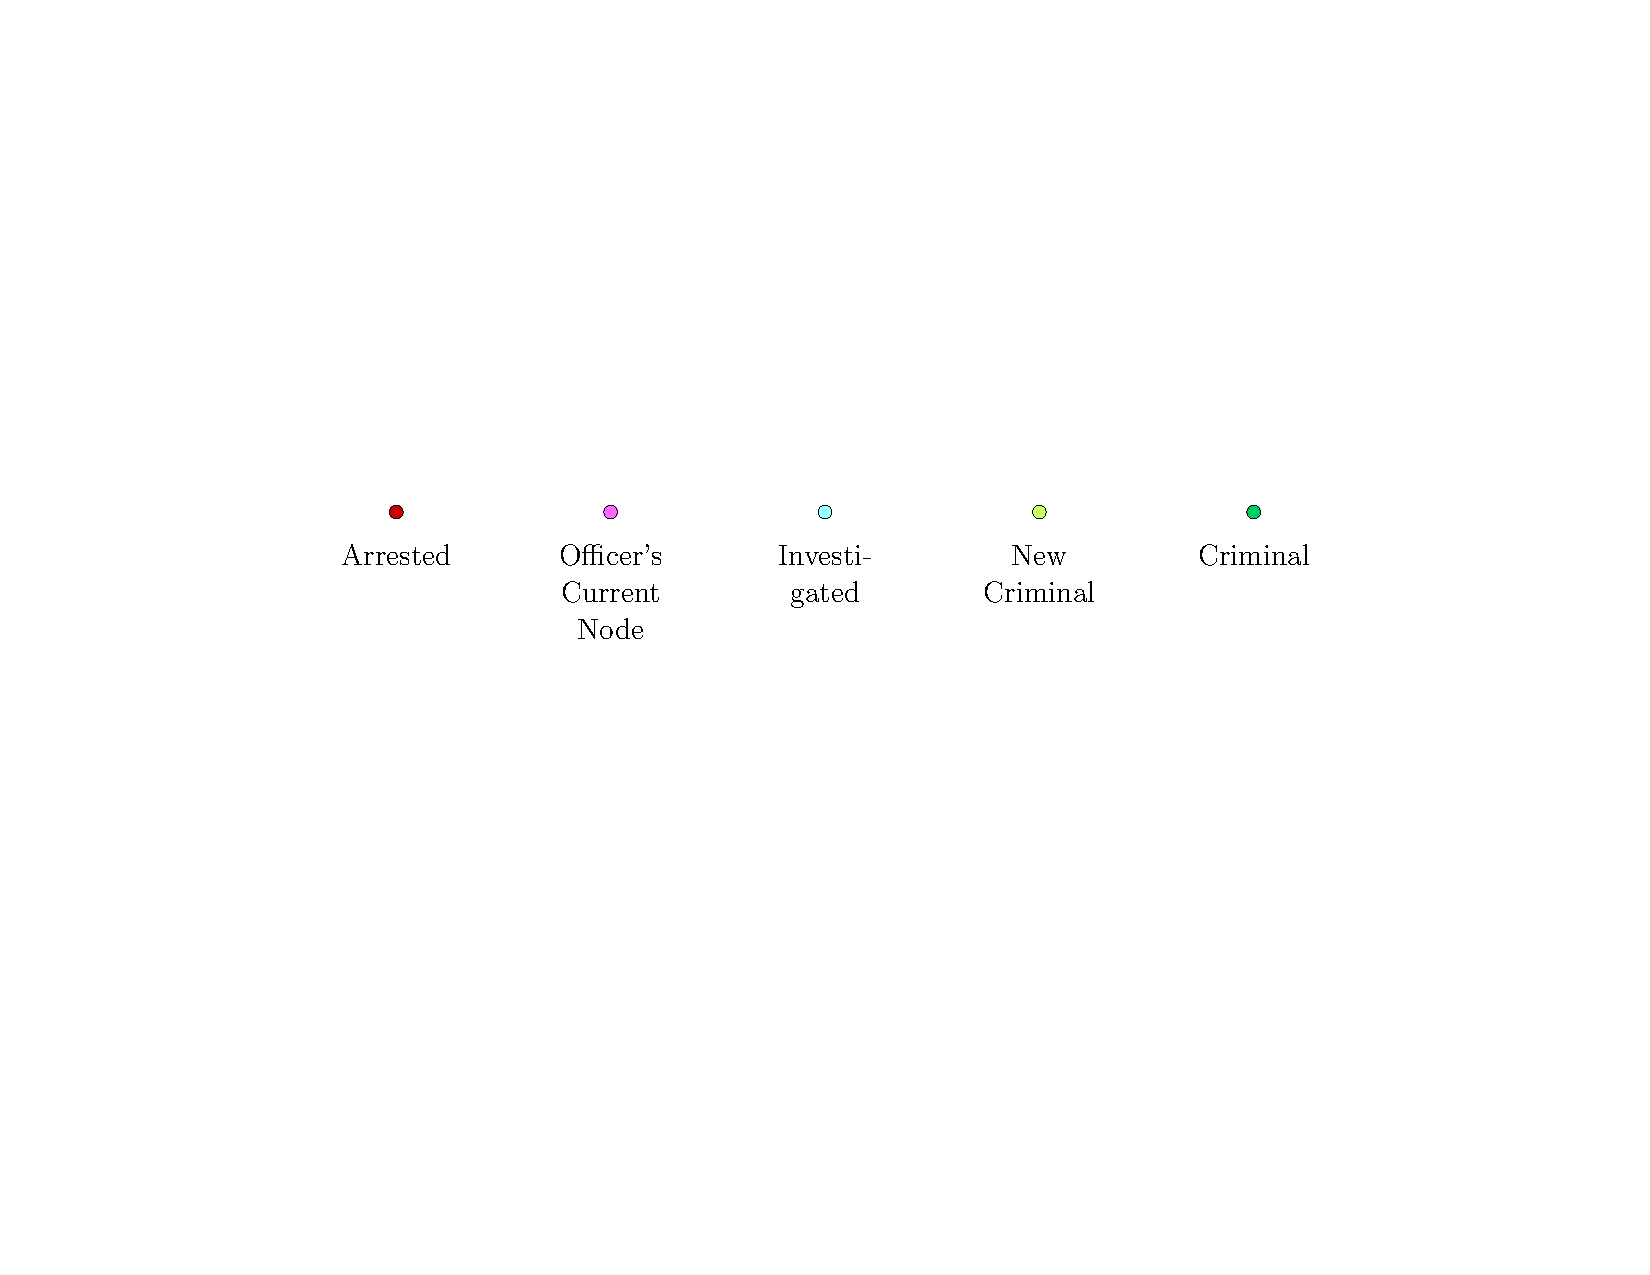
\includegraphics[width = .7\textwidth]{Key.pdf}
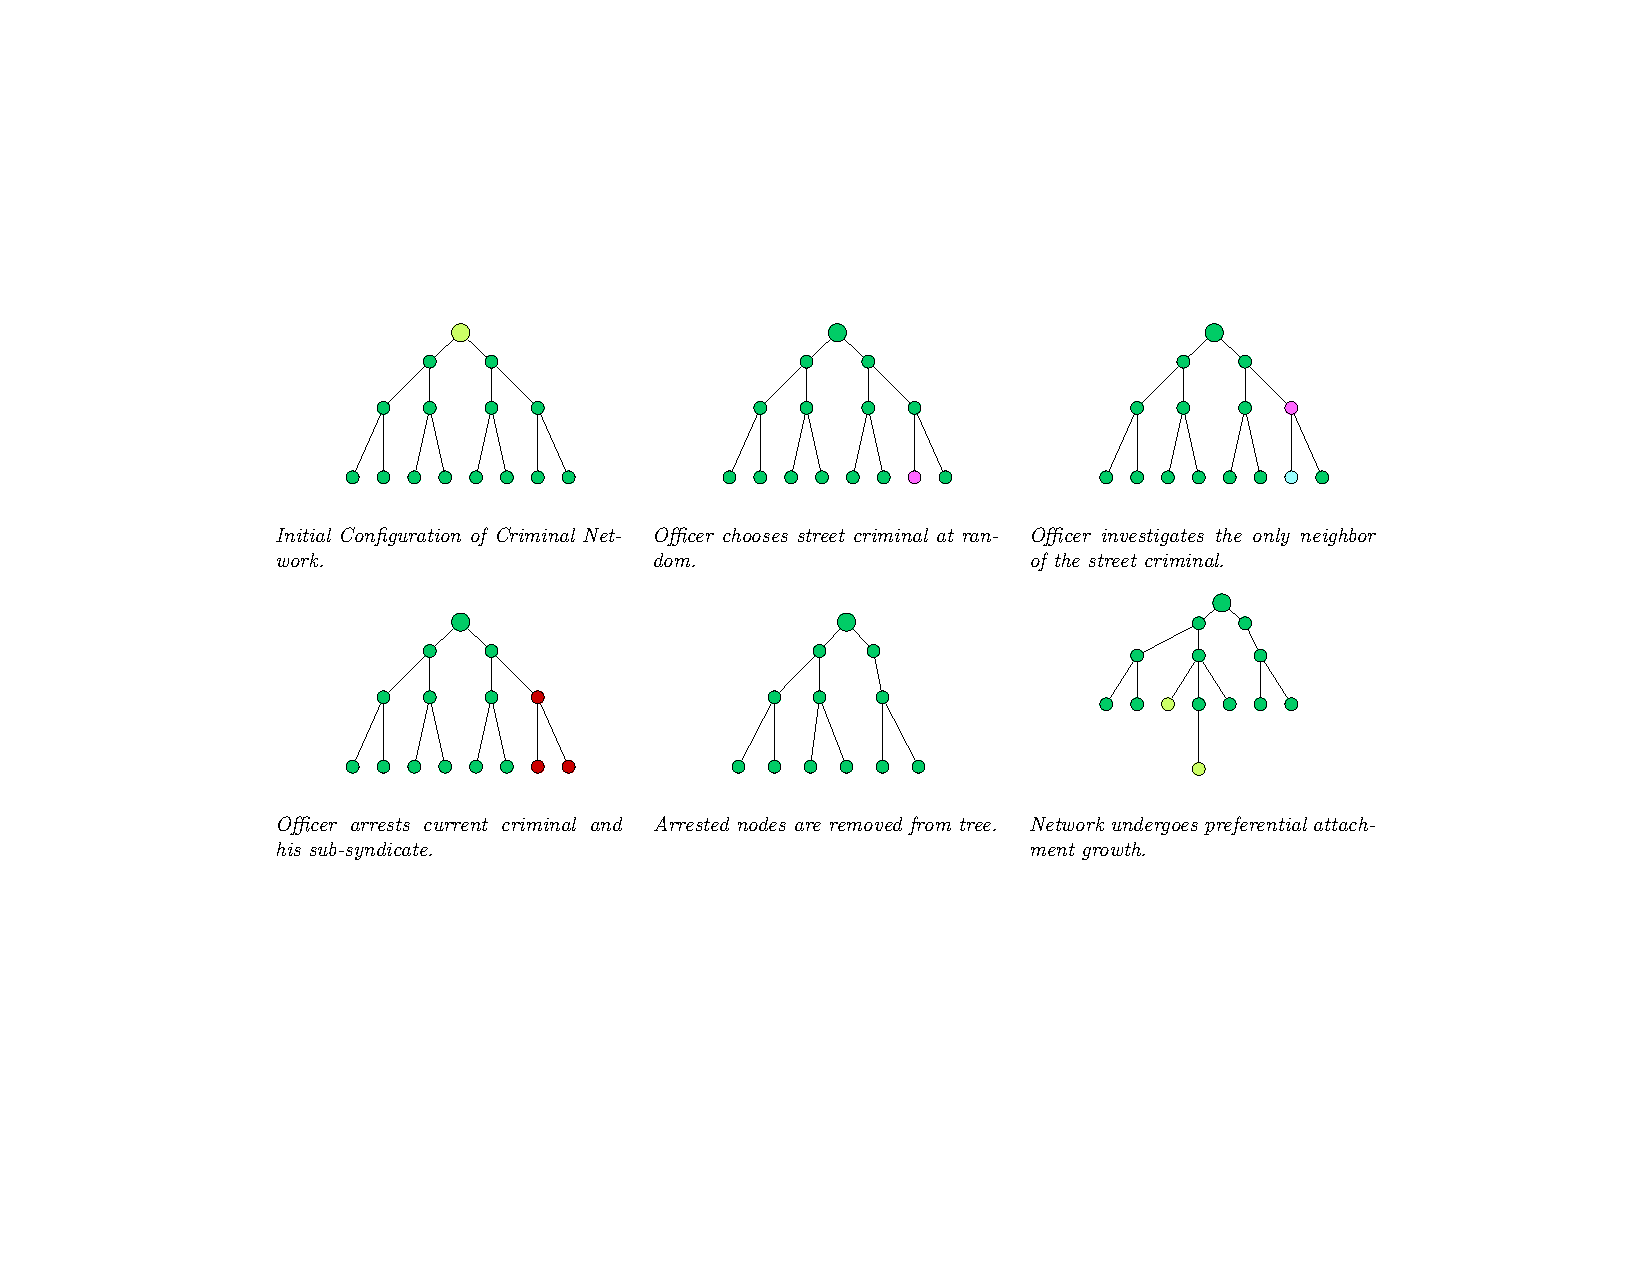
\includegraphics[width = \textwidth]{PursuitEvolution.pdf}
\caption{Above shows one iteration of the coupled pursuit and growth where the officer pursues strategy $S_A(1)$.  This strategy is when the officer investigates once and then arrests.  Here $k = 2$ for the growth process. }
\label{pe}
\end{figure}\\
\\
Let $S$ be the officer's strategy determining when she arrests a criminal during her investigation of the network.  We assess a strategy by calculating the maximum criminal arrival rate such that the officer wins with probability 1.  Let:
\begin{align*}
\textrm{Beat}(S) &:=\max\left(k \left| \substack{\textrm{police eliminate network in}\\ \textrm{finite time with probability 1}}\right.\right)
\end{align*}
The greater Beat$(S)$, the more effective a strategy $S$ is against a growing criminal network.  See Figure [\ref{beats}] for examples.

 \begin{figure}\centering
 \begin{subfigure}[b]{0.3\textwidth}
  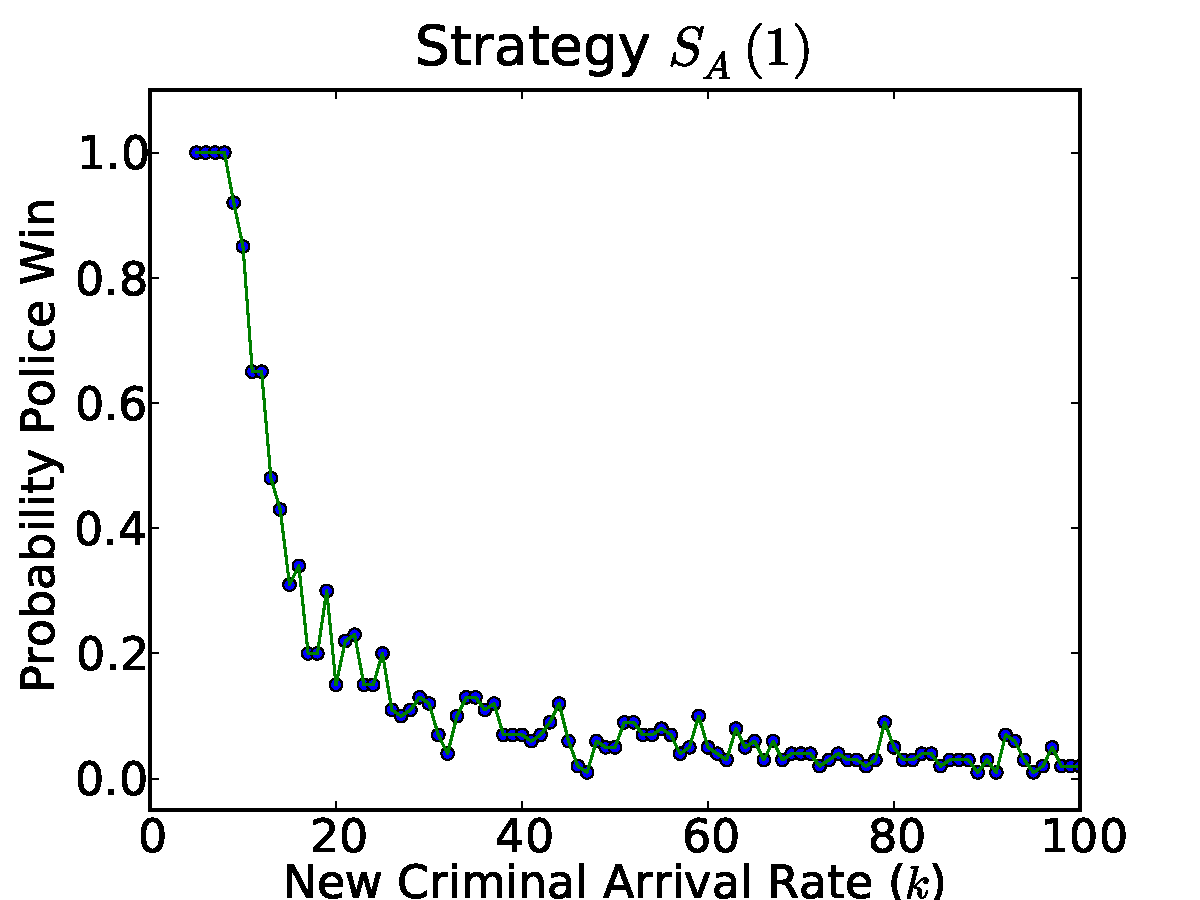
\includegraphics[width=\textwidth]{ImprovedPlotS0.pdf}
  \caption{}
  \end{subfigure}
   \begin{subfigure}[b]{0.3\textwidth}
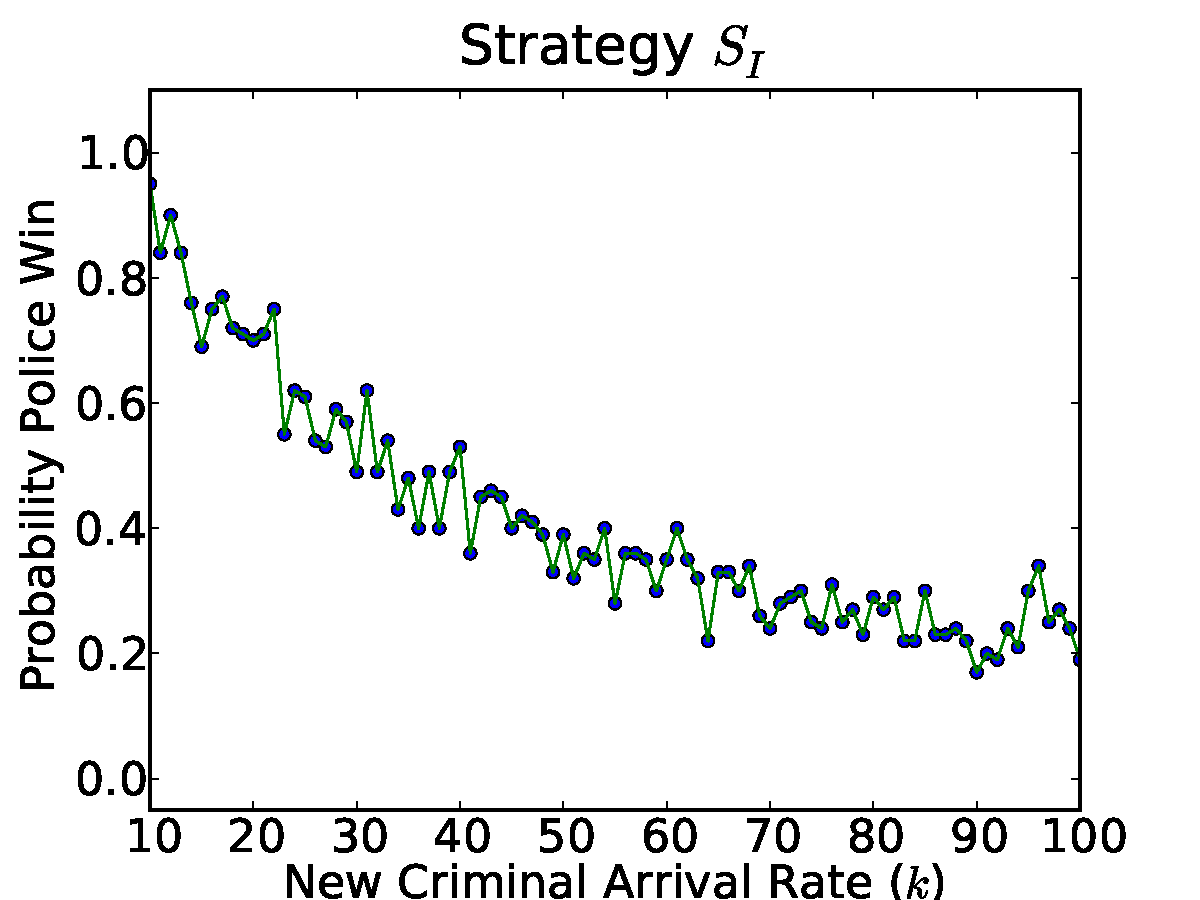
\includegraphics[width=\textwidth]{ImprovedPlotS1.pdf}
\caption{}
  \end{subfigure}
 \begin{subfigure}[b]{0.3\textwidth}
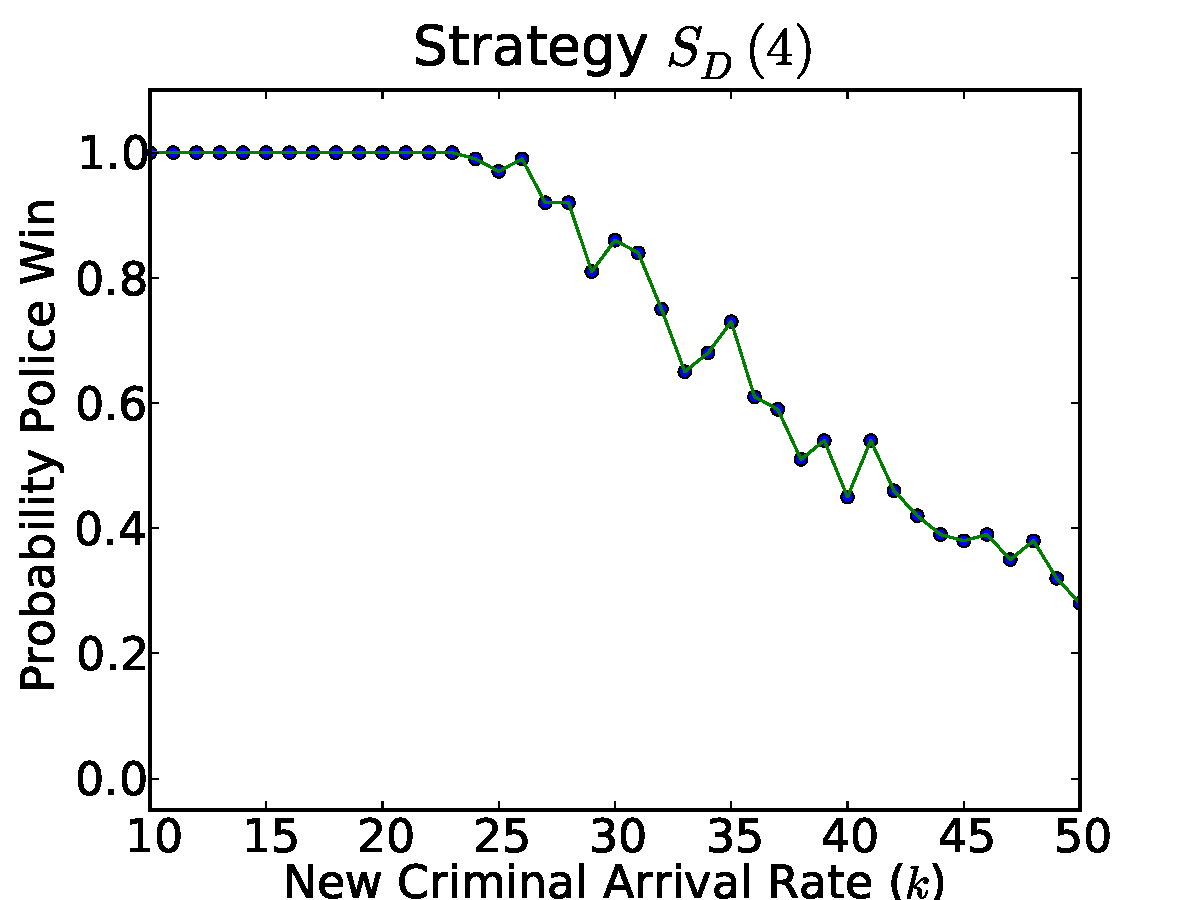
\includegraphics[width=\textwidth]{ImprovedPlotS3.pdf}
\caption{}
  \end{subfigure}

 \caption{We numerically determined the probability of winning with each strategy over 100 trials.  $S_A(1)$ plotted in $\b{(a)}$ is always successful for $k \leq 8$ and so we can estimate Beat$(S_A(1)) \approx 8$.  For $S_I$ plotted in $\b{(b)}$, there persists a non-zero probability that the root is caught even when $k$ is large, so the beat is small. Using $\b{(c)}$, we roughly estimate Beat$(S_D(4)) \approx 24$.}
 \label{beats}
 \end{figure}
 
 
 \section*{Simulations}
 
 We used NetworkX, NumPy, and SciPy for all the simulations.  Matplotlib and tike were used for the graphical representations.  The code for the preferential attachment tree, the dynamic game, and the experiments can be found at \url{here}.
 
\section*{Acknowledgements}
James von Brecht was instrumental in the early stages of this project including the foresight to implement these models in python.  This work was supported by grant X, Y, \& Z.





\bibliographystyle{unsrt}%Used BibTeX style is unsrt
\bibliography{bibliography}

\end{document}


%%%%%%%%%%%%%%%%%%%%%%%%%%%%%%%%%%%%%%%%%%%%%%%




%%%%%%%%%%%%%%%%%%%%%%%%%%%%%

